% TODO: Fix whitespace between word and units.
\section{The Silicon Tracker}
\label{sec:tracker}

At the heart of CMS is one of the world's largest silicon detectors: the silicon tracker, the closest sub-detector surrounding the interaction point.
The main goal of the silicon tracker is not to capture outgoing particles but to very precisely measure the hits from the charged particles as they pass through it.
The tracker also assists in vertex identification, differentiating between primary and secondary vertices, the latter of which often comes from B meson decays.
When multiple \pp collisions occur within the same BX (so-called \emph{pile up}), the tracker distinguishes between proton collisions with a resolution of about 100 \mum longitudinally and 50 \mum transverse to the beam pipe.
This is crucial to resolve which outgoing particles came from which \pp vertex.

The tracker consists of two types of pure silicon detectors: the pixel detector and the strip detector, each of which is described in turn below.
% , and are absolutely necessary to \emph{track} the decay products from \pp collisions.

% 100M pixels, 40M pictures per second.

\subsection{The Pixel Detector}
\label{sec:pixel}

The innermost part of the silicon tracker is the pixel detector, which is the closest subdetector to the interaction point.
The pixel detector is composed of 66 million silicon ``pixels'', as shown in Fig.~\ref{fig:tracker_real} (Left, pink).
A single pixel is 100\mum $\times$ 150\mum and, collectively, they cover a sensitive area of 1.9$\meter^2$.
Because it sits only 8\cm away from the beam pipe, the pixel detector receives the highest particle flux than any other subdetector:
around 10 million particles/$\cm^2$ per second.

The pixel detector is made of three cylindrical layers and two endcaps that surround the beam pipe.
In total, the pixel detector has around 6,000 connections (channels) per$\cm^2$.

After the LHC Run 1 was completed, the accelerator received luminosity upgrades during the 2013--2014 Long Shutdown.
To handle these higher luminosities, the pixel detector was replaced by the CMS Phase-1 pixel detector during the LHC technical stop in 2016--2017.
The upgrades outfitted the detector with four barrel layers and three endcap disks per side, which allowed for particle detection up to $\abseta < 2.5$.
The overall mass of the pixel detector decreased and granted the detector with better tracking capability.

% Cite:
% The CMS Phase-1 pixel detector upgrade
% To cite this article: W. Adam et al 2021 JINST 16 P02027
% https://d1wqtxts1xzle7.cloudfront.net/81437241/Adam_2021_J._Inst._16_P02027-libre.pdf?1645997389=&response-content-disposition=attachment%3B+filename%3DThe_CMS_Phase_1_pixel_detector_upgrade.pdf&Expires=1646800221&Signature=TRRZ5QLjlKL1rSOqgFxAMLY4vgj9EsI-NJSwy3erQAo2jhua1DZakAsJ-q1A4OB6KD1siSA20izwTEhzcojs8hhKZkC0y~gdcmxh7nrKDKmr59F8VMg2xINMemvOxyB9S3-pDxZN9t~VjtHhgAArmHmyLSuu90cy8BAFs3VkyZ1Wbr-RJx2uiRPb2zKXHWQw64laosnzKoBNvFg7B2ZdDaUpryDfPQpyZu3HkwQKV1Jd~ZpXlF0FjvxKm~QTm9Bk~bpxO5G5UiwaNv0sQhnWi37YAvs49yIks0NZrrCP7rbASStJ5L89sgSo44LPZxr3Usm6mGmglhW0eW8HliBYig__&Key-Pair-Id=APKAJLOHF5GGSLRBV4ZA


% REFERENCING THE CMS DETECTOR
% How Hualin has it:
% C. Collaboration, "the CMS Experiment at the CERN LHC," \textit{Journal of Instrumentation}, vol. 3, p. S08004, 2008.
% Compare the above to what gets printed out when you get bibtex working!

\subsection{The Strip Detector}
\label{sec:strip}

The outer part of the silicon tracker is called the strip detector, which has 10 million detector strips spread across 10 cylindrical layers.
The first 4 layers belong to the tracker inner barrel (TIB) and the remaining 6 layers belong to the tracker outer barrel (TOB), Fig.~\ref{fig:tracker_real} (Left, green and blue, respectively). 
Both the TIB and TOB have two endcaps associated with them, the TID and TEC, respectively.
Accounting for all of its components, the strip detector is sensitive to 200$\meter^2$.
Fig.~\ref{fig:tracker_xs} gives a clearly labelled transverse illustration of the pixel and strip detectors.
% It functions similarly to the pixels in that 
% It also has has slightly worse resolution than the pixel detector.
% Both the pixel and strip trackers have barrel and endcap components for nearly hermetic coverage around the beam pipe.
%%%%%%%%%%%%%%%%%%%%
\begin{figure}[h]
\centering
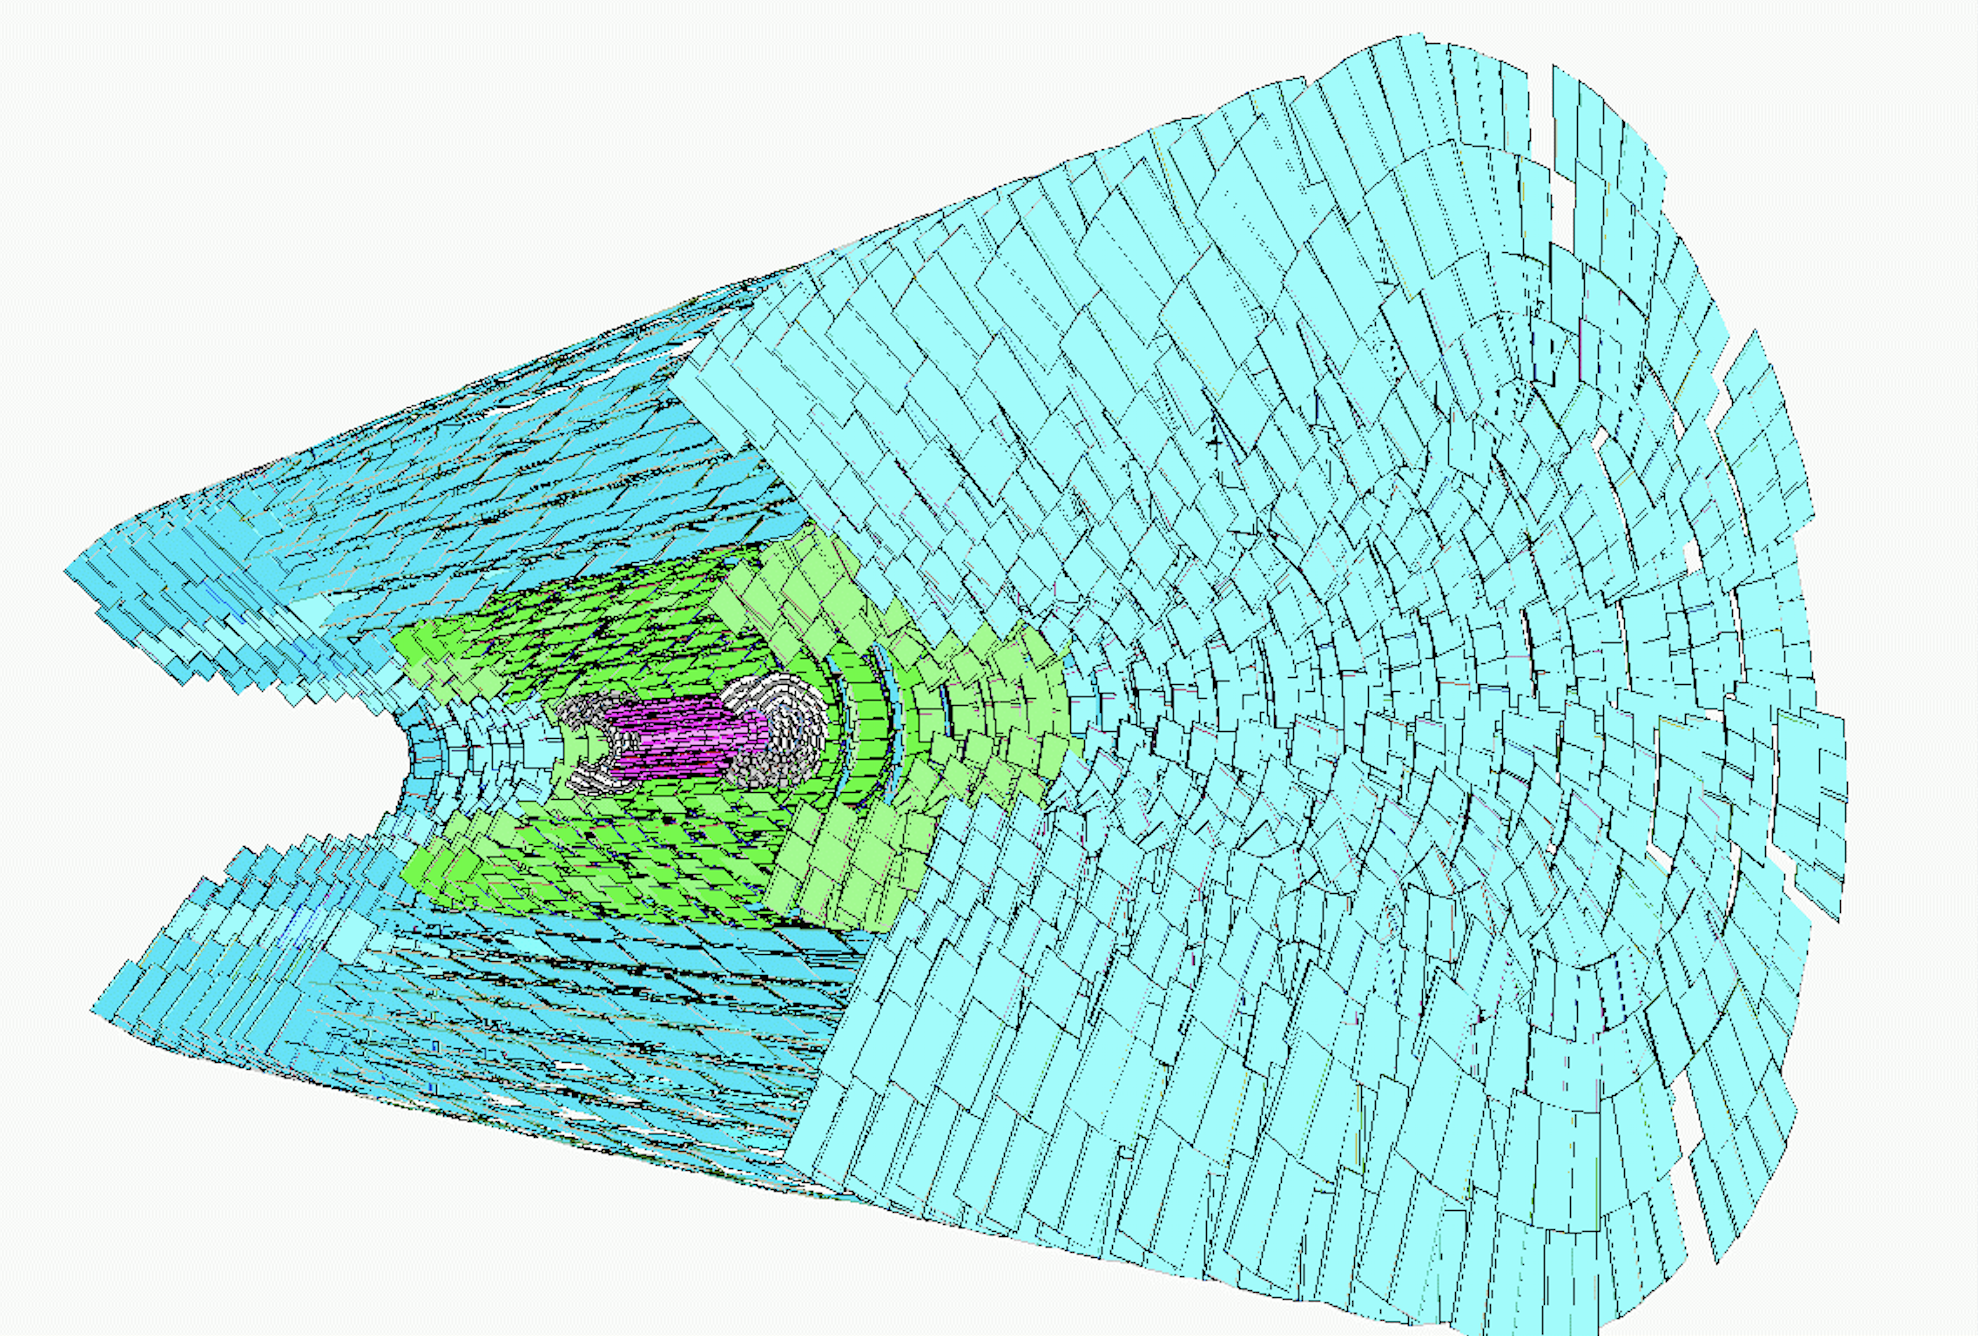
\includegraphics[width=0.49\textwidth,height=10cm,keepaspectratio]{figures/cms/tracker/silicon_tracker_simulated.png}
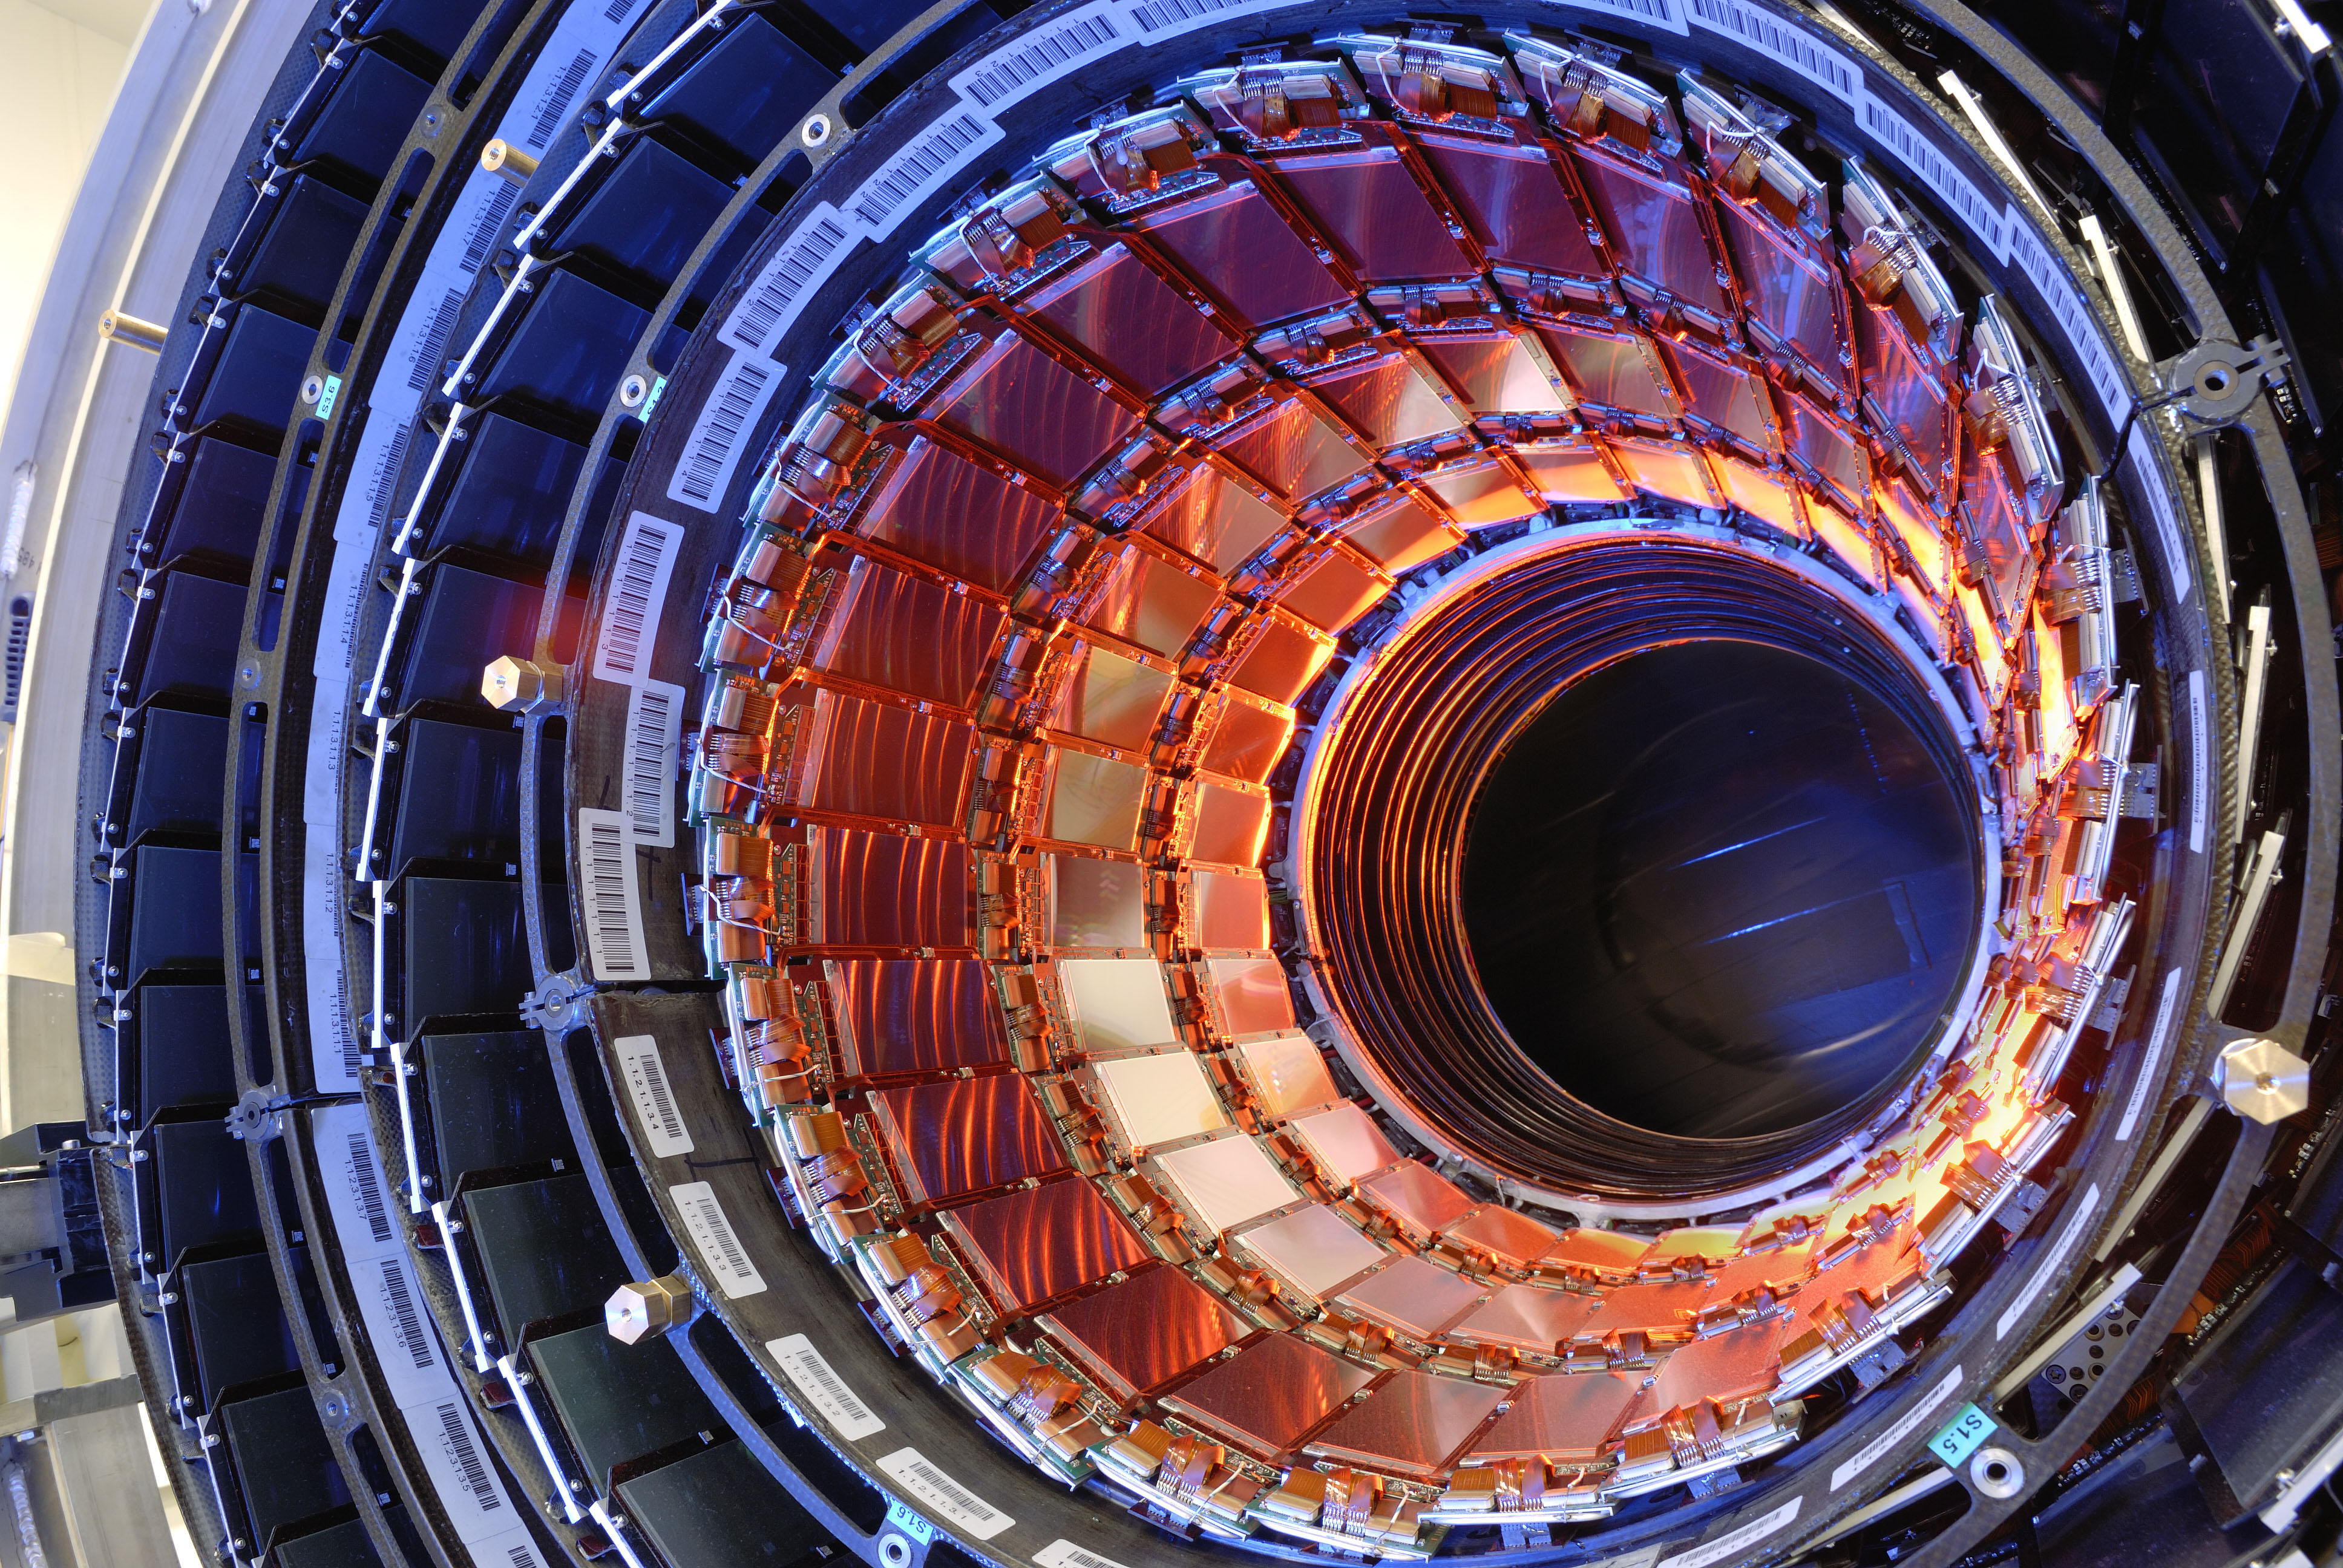
\includegraphics[width=0.49\textwidth,height=10cm,keepaspectratio]{figures/cms/tracker/silicon_tracker_real.jpg}
    \caption
        [(Left) A simulation of the silicon tracker. (Right) The real silicon tracker within CMS]
        {
        (Left) A simulation of the silicon tracker, showing the 3 cylindrical layers of the pixel detector (pink), 4 layers of the TIB (green), and the 6 layers of the TOB (blue) of the strip detector.
        The endcap components are also shown.
        (Right) A picture of the real silicon tracker at the center of CMS.
        } 
    \label{fig:tracker_real}
\end{figure}
%%%%%%%%%%%%%%%%%%%%
\begin{figure}[h]
\centering
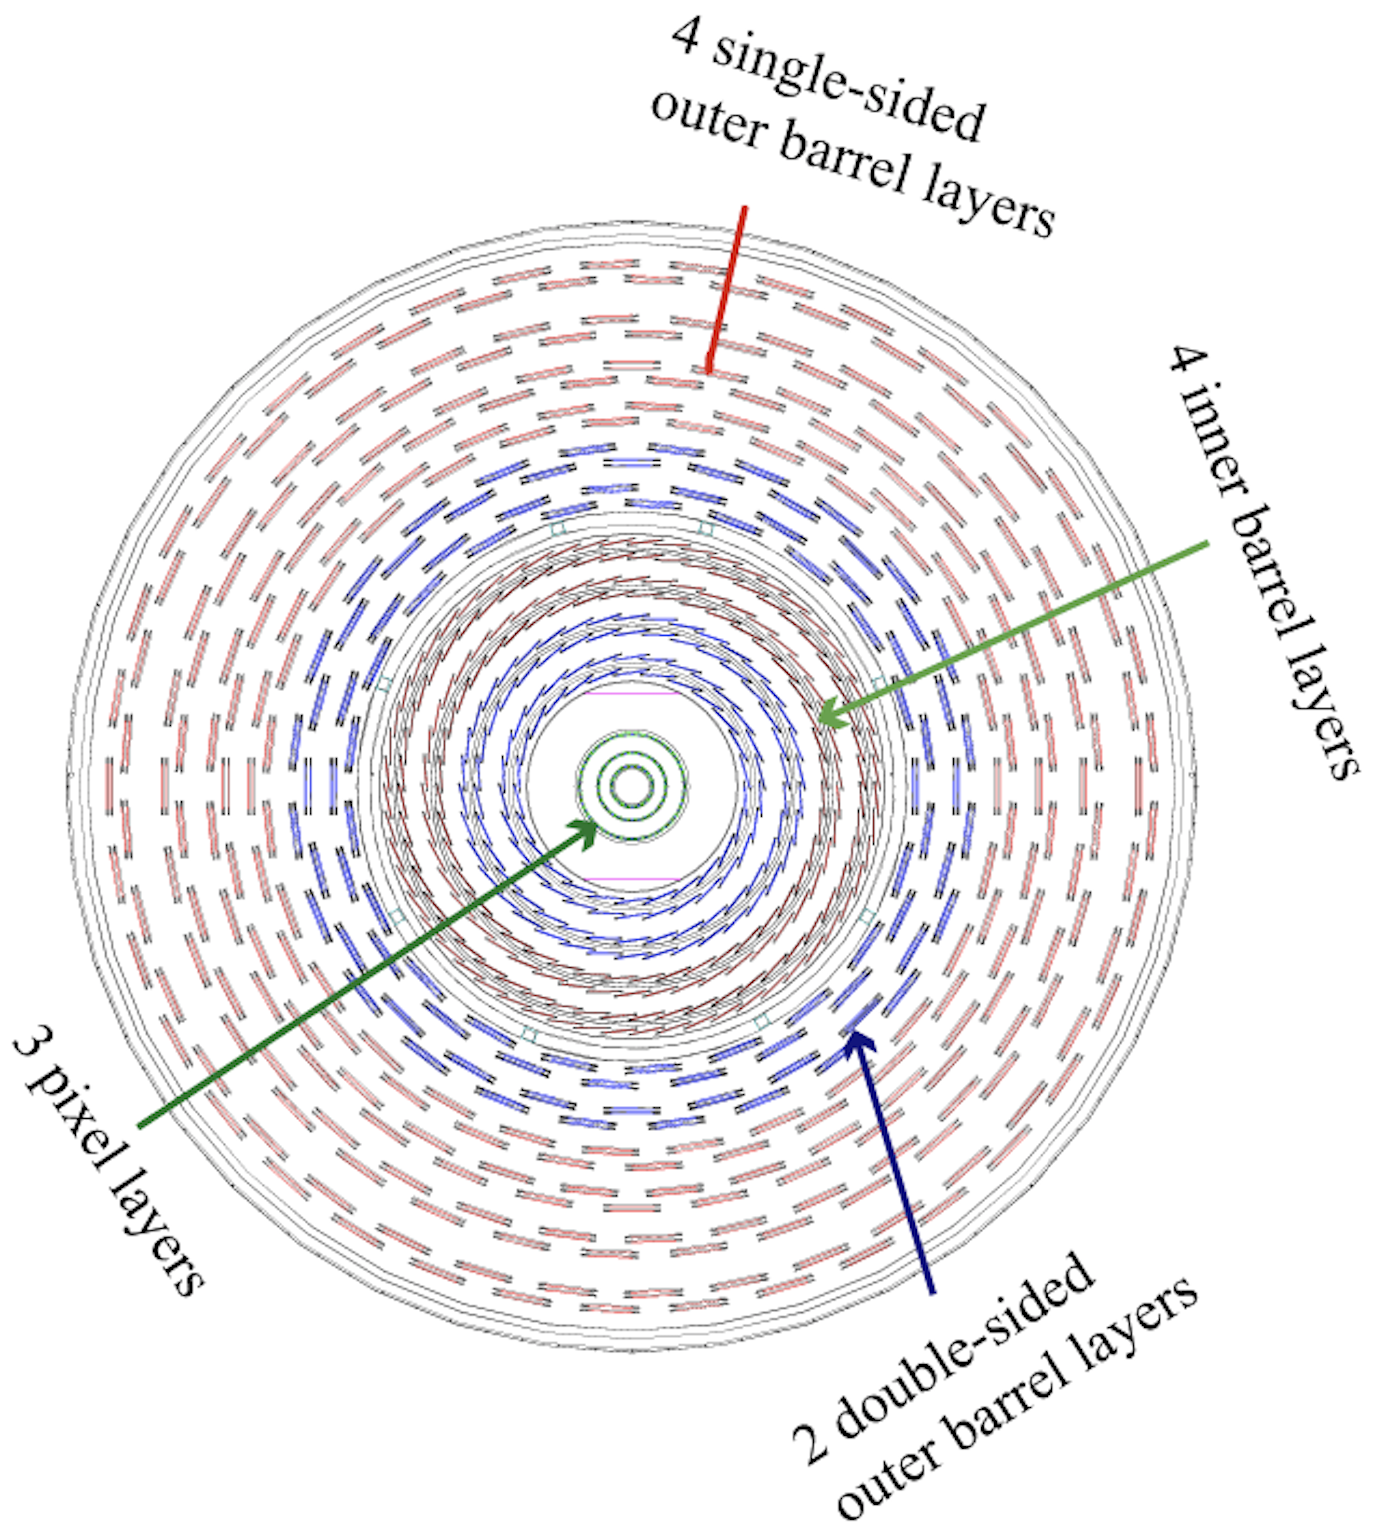
\includegraphics[width=10cm,height=10cm,keepaspectratio]{figures/cms/tracker/silicon_tracker_transverse_view.png}
    \caption{A transverse view of the silicon pixel and strip detectors, explicitly labelling the different layers involved.}
    \label{fig:tracker_xs}
\end{figure}
%%%%%%%%%%%%%%%%%%%%

% Consider the life of a particle produced from a \pp collision:
% Starting at the IP, the produced particles first have an opportunity to interact with the Tracker (Fig.~\ref{fig:tracker_real}, Right).
% Only charged particles will generate ``hits'' in the Silicon Tracker.
% Therefore, photons, neutrons, and neutral pions, \eg, are invisible to the tracker.
% Given enough hits and using sophisticated reconstruction software, we can determine precisely how the particle passed through the tracker.
% It's essentially a fancy game of ``connect-the-dots'' to determine the particle's trajectory.
% Figuring out the trajectory allows one to measure the radius of curvature, and therefore the momentum of the particle.
% This is what makes the Silicon Tracker such an important subdetector.

% Another major benefit of the Silicon Tracker is its assistance in vertex identification.
% During pile up (multiple proton collisions happening within the same BX),
% the tracker distinguishes between proton collisions with a resolution of about 
% 100~\mum longitudinally and 50~\mum transverse to the beam pipe.
% This is crucial to resolve which outgoing particles came from which \pp vertex.
% Since the tracker wasn't built to catch particles, they usually continue on to the next subsystems.
% Thus, CMS must be built as a kind of ``particle filter''.
% Electrons and photons are the first to be filtered out by the Electromagnetic Calorimeter...
